
\chapter{Vision}

Im Grunde geht es bei einem Editor für Flow Design vor allem darum die Vorteile aus der digitalen Welt mit
der Methodik zu vereinen, ohne die Einfachheit der Methodik auf dem Papier zu
      verlieren.

\section{Vorteile eines digitalen Editors}

Flow Design ist eigentlich als Entwurfsmethode auf dem Papier gedacht.
Jedoch hat ein Flow Design auf dem Papier einige Nachteile, die ein Editor am
Computer aufheben könnte. Das wären vor allem folgende Punkte:
\subsubsection{Einmal eingezeichnete Elemente lassen sich nicht mehr so leicht verändern.}

Während des kreativen Prozesses ein Programmierproblem zu lösen, bedarf es
mehrere Iterationen und Veränderungen an dem Diagramm. Eine Möglichkeit Versionen
abzuspeichern und Teile zu verschieben, umzubenennen und umzustrukturieren sind
klare Vorteile von einem digitalen Editor.
\subsubsection{Automatische Einhaltung der Notation}

Ein Editor bewirkt eine automatische Einhaltung der Notation.
\subsubsection{Automatische Validierungsprozesse}

Während der Erstellung des Flow Designs können im Hintergrund
Validierungsprozesse beim Erstellen des Diagrammes Hilfestellung bieten.
Autovervollständigungen könnten ebenfalls an einigen Stellen eingebaut werden,
um das Tippen zu beschleunigen.
\subsubsection{Unnötige Abtipparbeit ersparen.}

Aus den Beschriftungen im Flow Design Diagramm lassen sich die Variablennamen und
Methoden Signaturen leicht herleiten. Liegt das Diagramm in digitaler Form vor,
wäre eine automatische Generierung von Quellcode naheliegend und
würde dem Anwender unnötige Abtipparbeit ersparen. Außerdem können schnell
mehrere Iterationen eines Diagrammes erstellt und in
Versionskontrollsystemen eingepflegt werden.
Die Diagramme können auch einfacher von unterschiedlichen Orten aus und von mehreren
Personen abgerufen und bearbeitet werden.

\subsubsection{Generierung von Methodenrümpfe}

Durch die strikten Implementierungsregeln von Integrationen lassen sich für
diese Methoden nicht nur die Signaturen, sonder auch die komplette Implementierung aus dem Diagramm
ableiten. Eine Generierung dieser Codezeilen wäre ein zusätzlicher Komfortgewinn von einem Editor.
\subsubsection{Roundtrip-Engineering}

Eine Möglichkeit aus einer bestehenden Codebasis ein Diagramm zu erstellen -
wenn auch nur teilweise - würden die Produktivität beim Einsetzen von Flow
Design in einem Projekt weiter steigern.
Ein Anwendungsfall wäre: Der Anwender möchte
Teile seines Quellcodes in ein Flow Design überführen, um dann mit Hilfe des
Flow Designs, diesen zu überarbeiten und anschließend neu zu generieren.
Möglicherweise würde er die erstellten Codezeilen mit Copy\&Paste in sein
bestehendes Projekt übertragen.


\section{Vorteile von einem Entwurf auf dem Papier}

Ein Papier schränkt einen nicht ein und erlaubt es schnell und einfach Pfeile
und Kreise zu zeichnen, Notizen einzufügen und ist einfach in der Bedienung.
Bei dem Erstellen eine Editors muss deshalb ein besonders großes Augenmerk auf
eine gute und intuitive Bedienung gelegt werden, damit einem das Programm bei der kreativen Arbeit nicht
behindert. Endziel wäre es, dass der Anwender von sich aus lieber zum Editor
greift, als zu Stift und Papier, weil ihm der Editor komfortableres und
kreatives Arbeiten besser ermöglicht.

\chapter{Anforderungen}

Im Folgendem eine Auflistung der Anforderungen in Tabellenformat.

\section{Editor}

Die Anforderungen des Editors wurden aufgeteilt in drei Prioritäten: hoch, mittel und niedrig.

\begin{table}[H]
\begin{tabularx}{\textwidth}{X|l}
Anforderungen & Priorität\\
\hline \hline
Erstellen von Funktionseinheiten, Benennen, Verschieben auf dem Canvas, Löschen, Duplizieren & hoch\\ \hline
Navigation ( Panning, Zooming ) & hoch\\ \hline
Selektieren von mehreren Funktionseinheiten um mehrere auf einmal zu bearbeiten & hoch\\ \hline
Definieren von Eingangs- und Ausgangs-Datenströmen, für eine Funktionseinheit & hoch\\ \hline
Verbinden eines Ausgangs einer Funktionseinheit mit einem Eingang einer anderen & hoch\\ \hline
Zusammenlaufen/ Auseinanderlaufen von Datenflüssen (Joined- und Split-Notation ) & hoch\\ \hline
Funktionseinheit(en) einer anderen unterordnen können, um Integrationen zu erstellen inklusive visuelle Kennzeichnung & hoch\\ \hline
Speichern und Laden in ein Dateiformat & hoch\\ \hline
\end{tabularx}
\caption{Anforderungen mit hoher Priorität}
\end{table}

\begin{table}[H]
\begin{tabularx}{\textwidth}{X|l}
	Anforderungen & Priorität\\
	\hline \hline
Funktionseinheiten Klassen zuordnen & mittel\\ \hline
Syntaxhighlighting für die Datentypen auf den Datenflüssen & mittel\\ \hline
Keyboard Hotkeys / Tabstops & mittel\\ \hline
Automatisches Spacing & mittel\\ \hline
Validierung von Datenströmen & mittel\\ \hline
Untergeordnete Funktionseinheiten einer Integration an einer anderen Stelle definierbar machen, falls Platz knapp wird & mittel\\ \hline
Autosave & mittel\\ \hline
Undo / Redo System & mittel\\ \hline
Definieren von State einer Funktionseinheit & mittel\\ \hline
Definieren von neuen Datentypen & mittel\\ \hline
\end{tabularx}
\caption{Anforderungen mit mittlerer Priorität}
\end{table}


\begin{table}[H]
\begin{tabularx}{\textwidth}{X|l}

	Anforderungen & Priorität\\
	\hline \hline
Mouseover zeigt eine Vorschau des erzeugten Codes für die Funktionseinheit & niedrig\\ \hline
Wiederverwenden von vorhandenen Funktionseinheiten & niedrig\\ \hline
Autovervollständigung auf dem Textfeld der Datenströme & niedrig\\ \hline
Kommentarboxen & niedrig\\ \hline
Anfügen von Tests an Funktionseinheiten & niedrig\\ \hline
Mehrere Themes: Dark, Light (Print) & niedrig\\ \hline
\end{tabularx}
\caption{Anforderungen mit niedriger Priorität}
\end{table}



\subsubsection{Navigation}

Durch Inspiration aus Grafikanwendungen: Panning (Verschieben der Kamera in
der X- und Y-Achse) mit Hilfe der mittleren Maustaste. Zoomen in und aus dem
Diagramm durch das Mausrad. Die Position des Mauszeigers bestimmt das Zentrum des
Zooms.


\section{Generierung von Code}

Im folgenden eine Auflistung der Anforderungen einer Code-Generierung aus einem Flow-Design-Diagramm.

\begin{table}[H]
\begin{tabularx}{\textwidth}{X|l}
Anforderungen & Priorität\\
\hline
\hline
Generierung von Methodensignaturen anhand der ein- und ausgehenden Datenflüssen einer Funktionseinheit & hoch\\
\hline
Erzeugen des kompletten Methodenrumpfes einer Integration & hoch\\
\hline
Erzeugung von Klassen der benutzerdefinierten Datentypen & hoch\\
\hline
Einstellungen  dem Benutzer zugänglich machen, um die Generierung zu konfigurieren & mittel\\
\hline
Erzeugung von Namenspaces und Auflösung von Usings & niedrig\\
\hline
Korrektes Einfügen / Integrieren von den generierten Codezeilen in die Codebasis eines bestehendes Softwareprojektes & niedrig\\
\hline
Live-Generierung & niedrig\\
\hline
\end{tabularx}
\caption{Anforderungen der Code-Generierung}
\end{table}


\subsubsection{Erzeugung des kompletten Methodenrumpfes einer Integration}

Hierbei muss erkannt werden, in welcher Reihenfolge die Methoden aufgerufen
werden müssen, lokale Variablen erzeugt werden müssen und was einer Methode als Parameter
übergeben werden muss. Dabei kommen IEnumerables und Lambdas zum Einsatz um
Datenflüsse zu implementieren.

\subsubsection{Einstellungen für die Generierung dem Benutzer zugänglich machen
}
Mögliche Optionen wären:
\begin{itemize}
\item wie das Programm den Methodenrumpf einer Operation
standardmäßig befüllen soll: Leer, mit \textit{NotImplementedExeption} oder mit einem
Return-Ausdruck eines Standardwertes abhängig von der Methodensignatur.
\end{itemize}
\begin{itemize}
\item Ob innerhalb einer Integration der Rückgabewert einer Funktion erst in eine
lokale Variable gespeichert werden soll, oder direkt der Methodenaufruf an die
andere Methode weitergereicht wird. Beziehungsweise die Regel konfigurierbar
machen: Ab welcher Zeilenlänge, wie die Variablen benannt werden sollen, etc.
\end{itemize}

\subsubsection{Einfügen von generierten Codezeilen in bestehende Codebasis}

Notwendig hierfür wäre, dass bestehende Klassen gefunden werden müssten, Usings korrekt
eingefügt und schlussendlich die generierten Methoden und Datentypen in die
jeweiligen Klassen/Dateien eingefügt werden. Dabei muss die Syntax
berücksichtigt werden und möglicherweise Zugriffsberechtigungen erkannt und bei
Problemen einen Dialog zur Korrektur dem Anwender anbieten. Ein weiteres Problem
wäre die Überschneidung von Namen. Wenn automatisch der generierte Code bevorzugt
  werden soll, dann könnten durch die Überschreibung von Datentypen und Methoden
  bestehende Codezeilen plötzlich fehlerhaft werden. Ein extra Dialog wäre
  möglich, würde jedoch den Aufwand zur Integration des Codes möglicherweise stark
  anheben. Ebenso wäre ein solcher Dialog aufwendig zu implementieren.
 
  Eine andere Option wäre es, dies Codezeilen einfach einzufügen und die Erkennung und Lösung der
  Probleme der IDE zu überlassen. Gerade bei C\# gibt es mit Resharper viele
  Refactorisierungs-Tools, die einem bei der Lösung solcher Probleme unterstützen.



\section{Generierung von Flow Design Diagrammen aus Code}
\begin{table}[H]
\begin{tabularx}{\textwidth}{X|l}
Anforderungen & Priorität\\
 \hline \hline
Finden von Methoden und Erzeugen von Funktionseinheiten und ihre Datenströme anhand der Methodensignatur im Code & hoch\\ \hline
Automatisches Spacing & hoch ( aber nicht unbedingt perfekt)\\ \hline
Den Datenfluss einer Integration erkennen und ihn in ein Flow Design Diagramm übertragen & hoch\\ \hline
Erkennen, ob es sich bei der Methode um eine Operation oder Integration handelt & hoch\\ \hline
Umgang mit Methoden die nicht das IOSP befolgen & mittel\\ \hline
Speichern der Inhalte, die nicht im Diagramm dargestellt werden können. & mittel\\ \hline
\end{tabularx}
\caption{Anforderungen der Diagramm-Generierung}
\end{table}



\subsubsection{Automatische Anordnung}

Unbedingt notwendig, auch wenn es nur sehr rudimentär umgesetzt wird, ansonsten liegen
alle Funktionseinheiten nach dem Erstellen unübersichtlich auf einem Punkt aufeinander.
Falls das Automatische Spacing an manchen Stellen nicht perfekt funktionieren
sollte, kann eine gute Usability ( Selektierungs- und Verschiebungsfeatures)
hier dieser Imperfektion leichter verschmerzbarer machen.

\subsubsection{Schwierigkeiten}
Bei Verwendung von Events kann der Datenfluss möglicherweise nicht mehr nachvollzogen werden, da die \enquote{Verdrahtung} an beliebiger Stelle stattfinden kann und auch dynamisch zur Laufzeit.


\pagebreak
\chapter{GUI Skizzen / Usabilityüberlegungen}


\section{Minimalistischer Aufbau. Fokus auf Produktivität.}

Die Anwendung soll möglichst viel Platz für die Zeichenfläche
bieten.

\begin{figure}[H]
	\centering
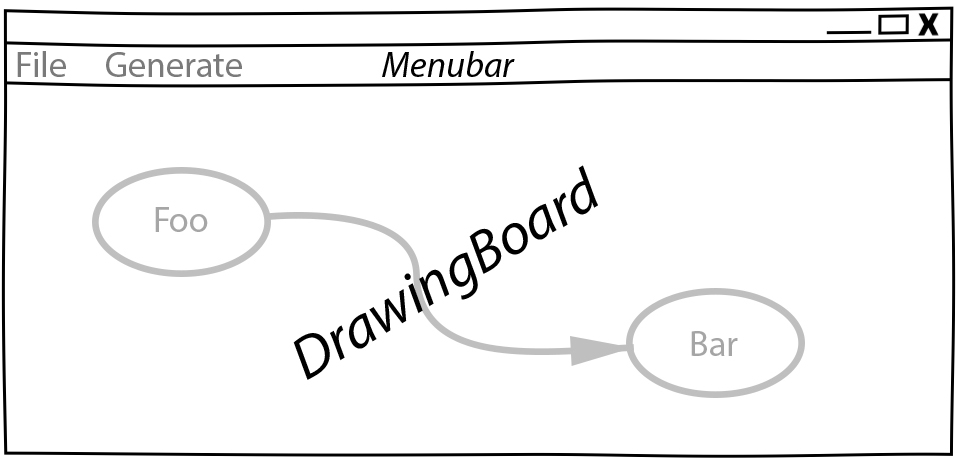
\includegraphics[width=.9\linewidth]{./img/MainCrop.jpg}
	\caption{Die Hauptansicht}
\end{figure}

Bei einem Rechtsklick auf eine leere Stelle in der Zeichenfläche erscheint ein Kontextmenu, dass dem Anwender erlaubt an dieser Stelle eine neue Funktionseinheit einzufügen.

\begin{figure}[H]
	\centering
	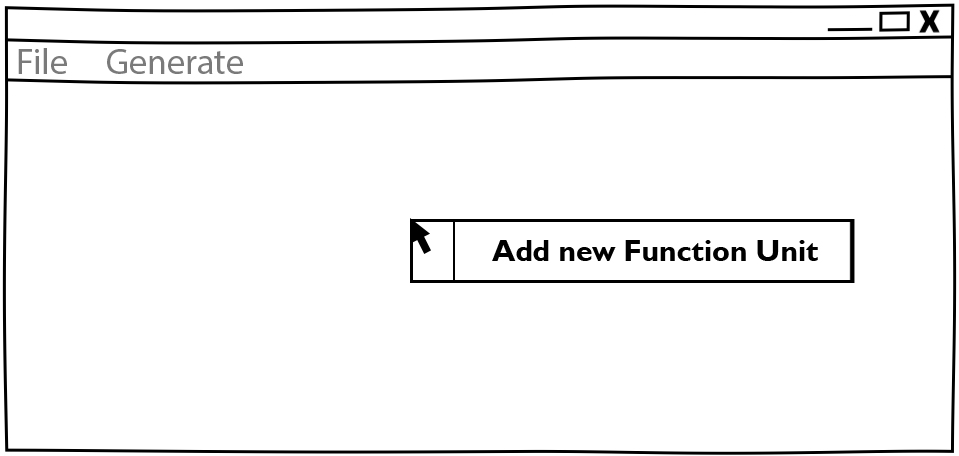
\includegraphics[width=.9\linewidth]{./img/ContextMenu.jpg}
	\caption{Ablauf einer Erstellung einer neuen Funktionseinheit}
\end{figure}


\begin{figure}[H]
	\centering
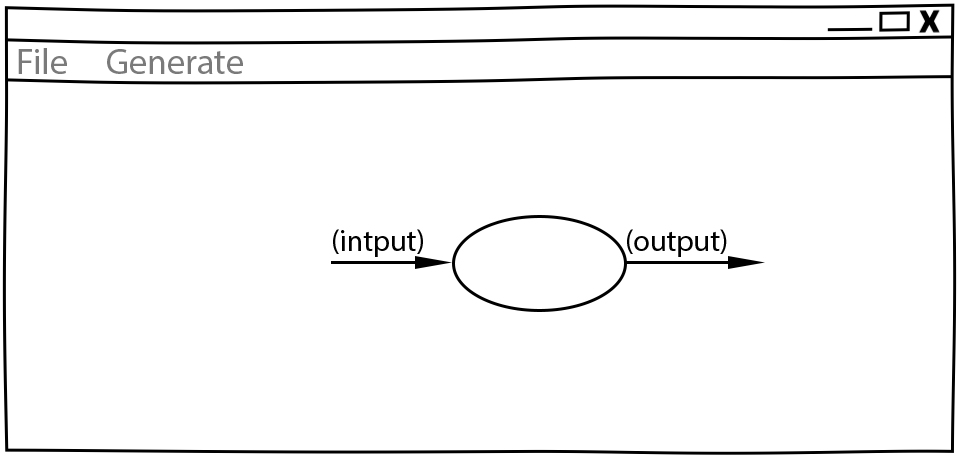
\includegraphics[width=.9\linewidth]{./img/NewCell.jpg}
	\caption{Eine neue Funktionseinheit wurde erstellt}
\end{figure}




\bigskip
Im folgendem einige Kerngedanken über die Funktionalität des Editors:

\begin{itemize}
\item Keine unnötigen Menüleisten, Symbolleisten, etc. besser kontextsensitive
Kontextmenüs, oder Tastenkürzel,  damit die Strecke, die die Maus bewegt werden muss, gering
gehalten wird.
\item Tabulatorstopps einbauen, damit schnell zwischen den Textfeldern, entlang des
Graphen, gesprungen werden kann.
\item Verwendung von Drag\&Drop, um eine intuitive Bedienung zum Verknüpfen von
Funktionseinheiten zu ermöglichen. Die Flächen, die per Drag\&Drop zu Bedienen
sind, sollen über ein Mouseover Feedback erkennbar sein. Außerdem sollen die
Flächen nicht zu klein sein, damit ein leichtes Treffen des Feldes
sichergestellt wird. Möglicherweise können auch unsichtbare Flächen verwendet
werden, um eine Drag\&Drop Fläche künstlich leicht zu vergrößern und einfacher treffbar zu machen.
\item Rectangle-Selection in Kombination mit Modifier-Keys um mehrere Funktionseinheiten
schnell und komfortable zu selektieren.
\item Shift + Drag : Schnelles Duplizieren der selektierten Elemente. 
\footnote{Vorbild dieser Funktion ist die CAD-Anwendung 3ds Max, das dieses Bedienkonzept an vielen Stellen einsetzt.
Einmal daran gewöhnt, möchte man es nicht mehr missen.} 

Anwendungsfälle:
Der Anwender möchte  schnell ein gesamtes Diagramm duplizieren und an ein andere Stelle schieben, um dort eine weitere Iteration davon zu erstellen.
Ein andere Anwendungsfall von Duplizieren ist, dass der Anwender eine vorhandene
Funktionseinheit an einer anderen Stelle im Diagramm verwendet möchte. 

\item Ctrl + Drag einer Funktionseinheit: Die Funktionseinheit und alle ihre Kinder werden
Verschoben. Anwendungsfall ist: Der Anwender möchte etwas Platz schaffen
zwischen zwei Funktionseinheiten. Mit einem Ctrl+ Drag der zweiten Funktionseinheit,
kann er diese und alle nachkommenden Funktionseinheiten verschieben, ohne sie
vorher extra selektieren zu müssen.
\end{itemize}

\section{Textfelder}

Textfelder müssen waagerecht bleiben. Auf dem Papier schreibt man die Daten auf
die Pfeile, somit wird Text auf einem schrägen Pfeil auch entlang des Striches
geschrieben.
Am Computer ist so etwas schlecht umzusetzen. Man kann Textfelder bei WPF drehen, dadurch
entsteht jedoch eine ungewohnte Bedienung beim Markieren von Text. Ein Drehen
beim Fokussieren/Defokussieren wäre auch möglich, damit wäre jedoch eine zusätzlicher
Klick nötig, falls man Text markieren möchte: Ein Mausklick zum Fokussieren/Drehen
der Textbox und ein weiterer um Text zu markieren / den Cursor zu platzieren.
Die beste Lösung wäre aus Usability-Sicht, wenn Textfelder nicht gedreht werden,
sondern immer waagerecht dargestellt werden. Somit muss hier die Notation an
manchen Stellen etwas vom original Abweichen.
\begin{itemize}
\item Mehrere Ausgänge
\item Pfeile zwischen zwei Funktionseinheiten, die auf unterschiedlichen Höhen platziert
sind.
\end{itemize}

\emph{Mehrere Ausgänge}



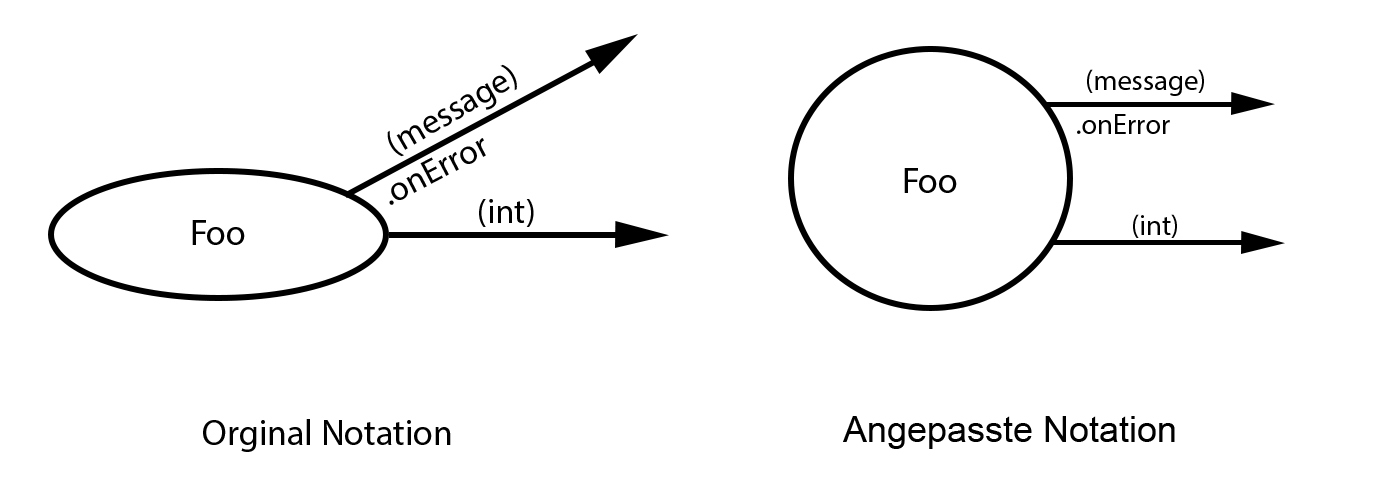
\includegraphics[width=.9\linewidth]{./img/NotationChanges1.jpg}
\bigskip

\emph{
Pfeile zwischen zwei Funktionseinheit, die auf unterschiedlichen Höhen platziert
sind}

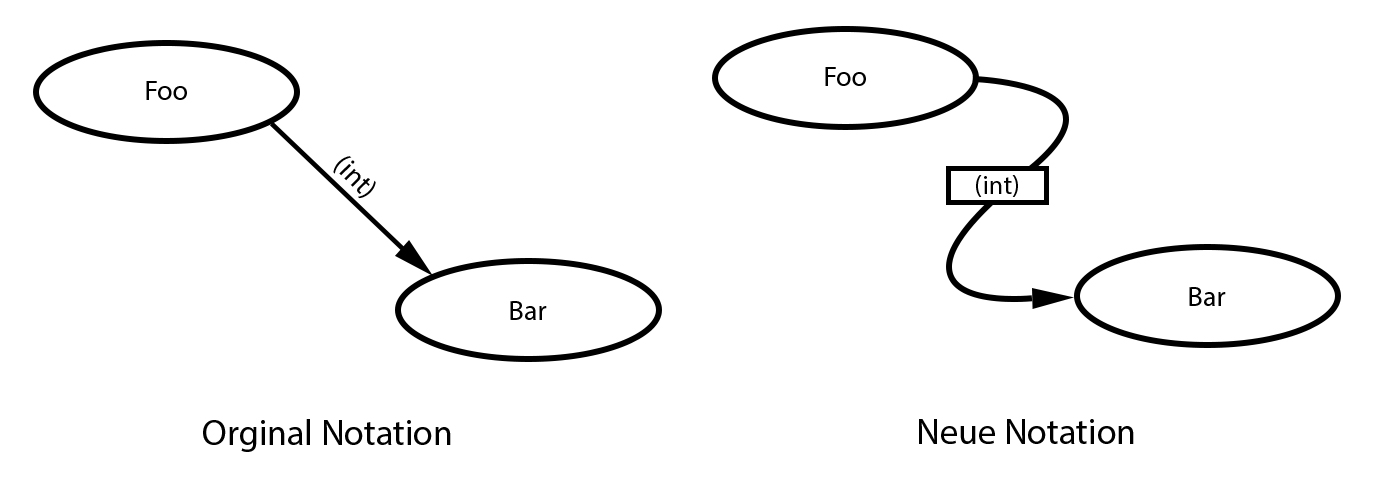
\includegraphics[width=.9\linewidth]{./img/NotationChanges2.jpg}



\section{Datentypen - Definition und Organisation}

Da Flow Design mit Datenströmen arbeitet, ist das Definieren neuer Datentypen
ein wesentlicher Bestandteil davon.
Eine Möglichkeit wäre es, wie auf dem Papier, es zu erlauben an beliebigen
Stellen im Diagramm eine Box zu erstellen, in der der Anwender einen neuen
Datentyp benennen und seine Felder definieren kann. Vorteil davon wäre, dass der
Anwender die nötige Information in der Nähe des Datenstroms schnell ersichtlich
platzieren kann, wo die Daten auch vorkommen.

Nachteil wäre, dass der Algorithmus zum automatischen Spacing komplizierter
werden würde, da nun auch eine sinnvolle Platzierung der Datentypen nun mit
berücksichtigen werden müsste.
Ein weiteres Problem dieser Lösung taucht auf, sobald der Anwender an unterschiedlichen
Positionen im Diagramm den selben Datentypen verwendet. In diesem Fall müssten Doppelungen erlaubt
sein, oder der Anwender würde an einer Stelle nicht die Information haben, worum
es sich bei einem Datentyp handelt.

Eine andere Option wäre es, die Datentypen nicht auf dem DrawingBoard zu
platzieren, sondern separate vom Flow Design getrennt in einem extra GUI-Element
darzustellen und dort die Definition eigener Datentypen zu ermöglichen.
Dieses GUI-Element würde in Form einer Liste alle vorhanden Datentypen
beinhalten. Zusätzliche Usability-Features wären, das Typen, die im Diagramm
vorkommen, jedoch nicht zu den Basistypen der Sprache gehören und noch nicht in
der Anwendung definiert wurden, erkannt und speziell hervorgehoben werden und
den Anwender subtil auffordert diesen zu definieren.

Um den Vorteil einer Box innerhalb des Diagrammes etwas zu entkräften, könnten
die Einträge in der Liste kontextsensitiv sein: Wenn der Anwender in ein
Textfeld eines Datenstromes klickt, könnte die Liste nur jene Datentypen
anzeigen, die in dem Textfeld vorhanden sind. Beim klick auf eine leere Fläche (
defokussieren des Textfeldes) würden wieder alle Datentypen im gesamten Diagramm
angezeigt werden. Des weiteren wäre eine visuelle Hervorhebung von nicht
verwendeten Datentypen auch denkbar.
\bigskip

\begin{figure}[H]
	\centering
	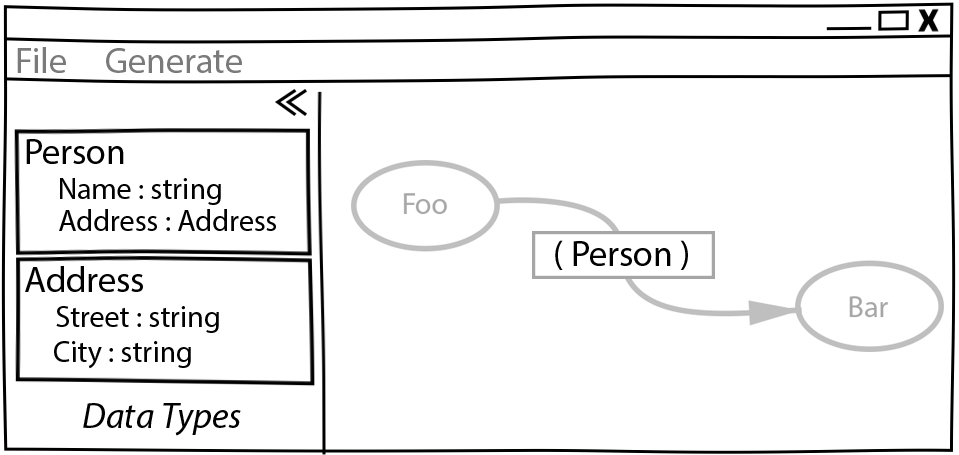
\includegraphics[width=.9\linewidth]{./img/DatatypesCrop.jpg}
	\caption{Datentypen Editor}
\end{figure}




Weitere Ideen: 
\begin{itemize}
\item Mouse-Hover über ein Datentype im Diagramm zeigt die Definition in einem Pop-Up
über dem Mauszeiger an.
\item Drag\&Drop von Datentypen aus der Liste in das \textit{DrawingBoard} zu
ermöglichen, falls der Anwender für einen Screenshot - oder aus einem anderen
Grund - diese Information im Bild haben möchte.
\end{itemize}


\section{Darstellung von Joined Inputs \& Split Outputs}

Datenströme können aus verschieden Quellen stammen und an einer Funktionseinheit
zusammenlaufen oder aus einer Quelle an viele andere Funktionseinheiten weitergereicht werden. Flow Design bietet hierfür die Pipe-Notation, oder die s.g. Joined Inputs und Split Outputs an. 

\bigskip

Vorteile der Pipe-Notation:

\begin{itemize}
\item Einfacher zu realisieren auf GUI Seite ( Automatisches Spacing aufgrund der
geringeren Anzahl an Pfeilen einfacher umzusetzen
\item Pfeile müssen seltener große Distanzen überbrücken, was das Diagramm weniger
chaotisch wirken lässt
\end{itemize}

Nachteile der Pipe-Notation / Vorteile der Joined Inputs \& Split Outputs:

\begin{itemize}
\item Datenströme sind möglicherweise nicht mehr eindeutig zu interpretieren. 
Bei der Verwendung von Joined Inputs ist die Herkunft eines Datenstroms eindeutig
ersichtlich. Bei der Pipe-Notation kann man diese Problem durch eine Benennung der Daten auf den Datenströmen lösen. Diese Erkenntnis legt eine Validierung - einschließlich visuellem Feedback - der Datenströme auf eine eindeutige Interpretation nahe.
\end{itemize}

Da beide Notationen ihre Vor- und Nachteile haben, soll die Anwendung beide Darstellungen unterstützen.

\section{Validierung des Datenflusses}

Der Validierungsprozess soll subtil sein. Ein Blockieren beim Verbinden zweier Funktionseinheiten soll nicht geschehen. Diese würde sonst dem Ziel entgegen stehen,
eine möglichst freie Gestaltung, wie beim Zeichnen auf dem Papier, zu
gewährleisten. Der Anwender soll die Freiheit haben, nicht valide Verbindungen
zu erstellen, die er möglicherweise erst nach dem Verbinden dann entsprechend
anpasst. Eine dezente farbliche Hervorhebung soll als Feedback des
Validierungsprozesses ( möglicherweise indem man den Pfeil einfärbt) ausreichen. Mögliche Validierungsfehler wären:
\begin{itemize}
\item Pipe-Notation : Überschneidung von Datentypen.
\item Fehlende Daten : Nicht alle vom Eingang der Funktionseinheit verlangten Daten
sind im Datenfluss enthalten.
\end{itemize}

Im Grunde wäre jedoch auch eine Generierung von jeglichen Flow Design Diagrammen
möglich, würde man folgende Regeln einführen:

Der Graph wird zurück gelaufen, bis ein passender Datentype
gefunden wird (das erste Vorkommen wird genommen). Falls der Datentyp nicht
gefunden wird, wird er in der Integration als lokale Variable deklariert und mit einem Standardwert initialisiert.


\section{Validierung der Syntax}

Die Notation der Daten der Datenflüssen besteht aus einer einfachen Syntax. Diese muss zwingend eingehalten
 werden, damit eine Generierung des Codes möglich ist.
 Eine rote gewellte Linie unterhalb des nicht validen Textes soll dem Anwender
 anzeigen, dass ein Syntaxfehler vorhanden ist.

